\documentclass{article}
%\documentclass[prl,amsmath,amssymb]{revtex4} % PRL

% margins of 1 inch:
\setlength{\topmargin}{-.5in}
\setlength{\textheight}{9in}
\setlength{\oddsidemargin}{0in}
\setlength{\textwidth}{6.5in}

\usepackage[pdftex]{hyperref} % hyperlink equation and bibliographic citations
\usepackage[dvips]{graphicx,color}
\usepackage{amsmath} % advanced math
\usepackage{verbatim}
\usepackage{natbib} % bibilography 
\usepackage{mciteplus} % collapse multiple citations in bibilography
\usepackage{multicol}
\usepackage[toc,page]{appendix} % http://tex.stackexchange.com/questions/49643/making-appendix-for-thesis


% from http://www.flakery.org/search/show/569
%\newcommand{\infint}{\ensuremath{\int_{-\infty}^{\infty}}}
\newcommand{\cf}{\textit{c.f.}} % "compare". In context the abbreviation advises readers to consult other material, drawing attention to related ideas that provide additional arguments or information.
\newcommand{\ie}{\textit{i.e.}} % i.e. is used to explain, clarify or rephrase a statement
\newcommand{\eg}{\textit{e.g.}} % “for the sake of example”. Used to introduce an example or list of examples to illustrate what is being discussed.
\newcommand{\eqn}[1]{Eq.\ (\ref{#1})}
\newcommand{\pfrac}[2]{\ensuremath{\frac{\partial #1}{\partial #2}}}

\begin{document}
\title{Introduction to the Physics Derivation Graph}

\author{Ben Payne$^{1}$\footnote{Corresponding author: ben.is.located@gmail.com}, Michael Goff$^{2}$\\
{\it $^{1}$Department of Fun, University Name \& Town, city, State Zip}\\
{\it $^{2}$Department of Mathematics, University of Maryland \& Baltimore 21228}}

\date{\today}

%\begin{abstract}
%blah blah blah
%\end{abstract}

\maketitle % declares end of title page
\begin{multicols}{2}

%\tableofcontents

%\newpage

% Introduction: scope = ?

\section{Introduction}

% relevant project background
The Physics Derivation Graph is a project designed to capture mathematical physics knowledge. 

Historically, knowledge about physics has been recorded in the form of notes, letters, journal articles, and text books. The content is typically composed of text, equations, and pictures. The presentation is in a linear sequence, though references are made to link the current section with previous sections and later sections. 

A recent addition has been the use of webpages to capture knowledge. A primary example of this is Wikipedia, an HTML-based encyclopedia. Webpages such as Wikipedia still use text, equations, and pictures, but add a distinct capability: hyperlinks. Hypertext Markup Language offers the ability to connect content to any other content. This enables non-linear exploration of content, in contrast to a textbook which is designed to be read sequentially. 

The Physics Derivation Graph is a non-linear capture of knowledge with mathematically-based links of physics content. A graph is composed of node and edges. This graph has two types of nodes: mathematical statements and inference rules. Every mathematical statement (referred to here as a statement) is connected to an inference rule by a directed edge. An example is provided which illustrates the concepts.

Frequency $f$ and period $T$ are related by
\begin{equation}
T\ f = 1
\label{eq:period_and_freq}
\end{equation}
Thus, frequency in terms of the period is
\begin{equation}
f = 1/T
\label{eq:freq_is_inverse_period}
\end{equation}
The relation between \eqn{eq:period_and_freq} and \eqn{eq:freq_is_inverse_period} is that both sides of \eqn{eq:period_and_freq} were divided by $T$. 

In the above example, there are two mathematical statements: \eqn{eq:period_and_freq} and \eqn{eq:freq_is_inverse_period}. These statements are related by an inference rule: ``Divide both sides of first equation by a value to yield the second equation.'' This inference rule takes an argument, referred to here as the ``feed'', which in this example is $T$. This set of steps is shown graphically in~Fig.~\ref{fig:freq_period}

\begin{center}
\begin{figure}
%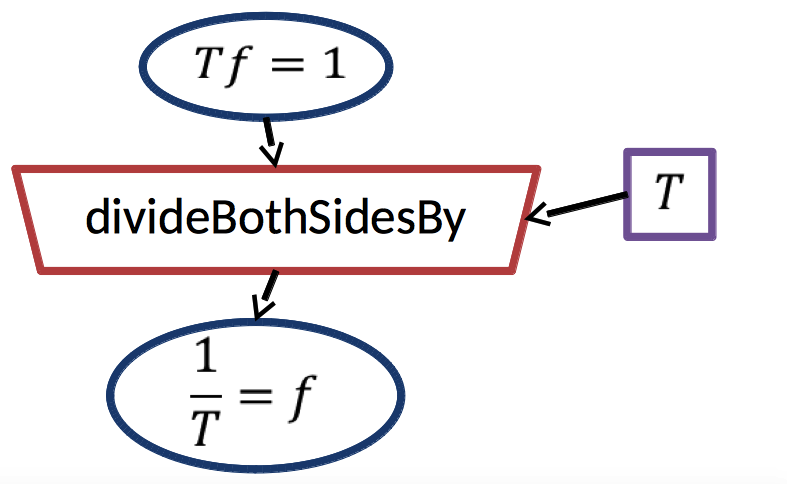
\includegraphics[scale=1]{images/frequency_period_relation.png}
\caption{Relation between period $T$ and frequency $f$.\label{fig:freq_period}}
\end{figure}
\end{center}
\section{Development Stages}

This project is expected to evolve through distinct steps. Each step can be characterized by different users and associated requirements. 
% \subsection{Gathering Examples}
The first step is prototyping and has a small number of expert users interested in gathering content for the Physics Derivation Graph. This exploratory phase involves research on appropriate syntax for the graph, brainstorming use cases, and minimal interaction with an external community. 

% \subsection{Proof of Concept}
The second phase is when sufficient examples exist to constitute a proof of concept. This requires breadth of coverage across all the domains of physics (\ie, classical mechanics, quantum mechanics, relativity, thermodynamics, statistical mechanics, etc). As a consequence, much of mathematics covered up to undergraduate level is likely to be required. 

% \subsection{Interface Creation}
Once the breadth of coverage is demonstrated, the next step is to enable development of indepth creation for the Physics Derivation Graph. Currently, content is manually entered into an XML database, and visualization of the graph is generated via the command line. To make both data entry and visualization more accessible to users and developers, a web browser-based interaction is planned. 

% \subsection{Community Utilization}
The most difficult step may be adoption and utilization by the scientific and education communities. This widespread use is dependent on having useful and reliable content, intuitive interfaces, and addresses a need. The Physics Derivation Graph does not currently exist, implying the needs being addressed are either unclear or sufficiently complex to make solution difficult. 

The steps listed above are sequential, but will likely be worked on concurrently. Exploration of an intuitive interface can take place while examples are being gathered. In the next section, use cases which motivate users of this project are described. 

\section{Use Cases}

While curiosity has driven the development of the Physics Derivation Graph, the resulting work is expected to be useful to multiple audiences and users. Viewers of the content could include students in math and physics, and analysis of the content could help shape curriculum. Contributors to the Physics Derivation Graph would be scientists who add new developments based on their work.

\subsection{Students in Math and Physics}

Currently students in Math and Physics are taught content using lectures, textbooks, and homework. The method of presentation varies, but the overarching story is often historically driven. Algebra is old, calculus is newer, and topology is recent. Classical mechanics is old, thermodynamics is newer, and quantum mechanics is recent. When teaching, these subjects are taught by building on previous content -- calculus leverages algebra, thermodynamics leverages classical mechanics. 

\subsection{Scientific Articles}

Peer-reviewed journal articles are one of the current methods of demonstrating value in the scientific community. Conciseness is a feature of this writing style, and the mathematics presented is correspondingly sparse -- just sufficient to covey the author's intention. This results in a burden on the reader of the article, either to take the author's claims on faith, or to rederive the mathematical statements. A reader's derivation is complicated by implicit assumptions made by the author and unintentional mistakes in calculation. 

With journals allowing supplemental materials for articles, calculations could be included. However, it is not clear what the appropriate level of detail is in supplied calculations. The intention is to be able to reproduce the work, but 

validation via computer 

\subsection{Education Curriculum Design}

A less direct use case but potentially important impact of the Physics Derivation Graph is on understanding the relevance of what is being taught in the education system. Math classes essentially teach a set of inference rules, and physics is the application of those inference rules. The Physics Derivation Graph could answer two important questions: ``When am I going to use this inference rule?'' and ``What's the relative importance of this math skill?''

The focus for students in mathematics classes is on the technique, \ie, ``integrate both sides with respect to $Y$,'' and application is necessarily of secondary importance. Physics students are expected to know the mathematical techniques and teaching is focused on application. The Physics Derivation Graph can assist both scenarios. The student in a math class can see where the inference rules they learn are applied in Physics. The student in the Physics class can see which inference rules are required in their field. 

Each inference rule seems equally important, since it currently isn't known what the frequency of use for that inference rule is. From the Physics Derivation Graph, it is simple to count utilization of inference rules. Thus, we are able to measure the ratio of how often ``multiply both sides by X'' is used relative to ``integrate both sides with respect to $Y$.'' 

\section{Bibliography}

\bibliographystyle{unsrt}
\bibliography{../bibliography} % external bibtex flat-file database
\end{multicols}

\newpage
\appendix
%\begin{appendices}
%\section{Test cases in Latex and MathML}\label{sec:appendix_test_cases}

\subsection{Case 1: polynomial}

\begin{equation}
a x^2 + b x + c = 0
\label{eq:polynomial_case1}
\end{equation}
Latex: 
\begin{verbatim}
a x^2 + b x + c = 0
\end{verbatim}

SymPy:
\verbatiminput{sympy_case1_polynomial.py}

Presentation MathML:
% http://www.mathmlcentral.com/Tools/FromMathML.jsp

%\begin{figure}
%\begin{center}
%\includegraphics[scale=1,bb=0 0 111 19]{images/case1_polynomial_mathML_presentation.gif}
%\caption{Case 1 polynomial in Presentation MathML}
%\end{center}
%\end{figure}

\verbatiminput{mathML_presentation_case1_polynomial.xml}

Content MathML:
\verbatiminput{mathML_content_case1_polynomial.xml}

\subsection{Case 2: Stoke's theorem}
\begin{equation}
\int \int_{\sum} \vec{\nabla} \times \vec{F} \dot d\sum = \oint_{\partial \sum} \vec{F}\dot d\vec{r}
\label{eq:stokes_case2}
\end{equation}
Latex:
\begin{verbatim}
\int \int_{\sum} \vec{\nabla} \times \vec{F} \dot d\sum = 
\oint_{\partial \sum} \vec{F}\dot d\vec{r}
\end{verbatim}

SymPy:
\verbatiminput{sympy_case2_stokes.py}


Presentation MathML:
\verbatiminput{mathML_presentation_case2_stokes.xml}

Content MathML:
\begin{verbatim}
<math xmlns="http://www.w3.org/1998/Math/MathML">

</math>
\end{verbatim}

\subsection{Case 3: Tensor analysis}
\begin{equation}
Y^i(X_j) = \delta^i_{\ j}
\label{eq:tensor_analysis_case3}
\end{equation}
Latex: 
\begin{verbatim}
Y^i(X_j) = \delta^i_{\ j}
\end{verbatim}

SymPy:
\verbatiminput{sympy_case3_tensor.py}


Presentation MathML:
\verbatiminput{mathML_presentation_case3_tensor.xml}

Content MathML:
\begin{verbatim}
<math xmlns="http://www.w3.org/1998/Math/MathML">

</math>
\end{verbatim}


\subsection{Case 4a: creation operator}
\begin{equation}
\hat{a}^+ |n\rangle = \sqrt{n+1} |n+1\rangle
\label{eq:creation_operator_case4a}
\end{equation}

\begin{verbatim}
\hat{a}^+ |n\rangle = \sqrt{n+1} |n+1\rangle
\end{verbatim}

SymPy:
\verbatiminput{sympy_case4a_creation.py}


Presentation MathML:
\verbatiminput{mathML_presentation_case4a_creation.xml}

Content MathML:
\begin{verbatim}
<math xmlns="http://www.w3.org/1998/Math/MathML">

</math>
\end{verbatim}

\subsection{Case 4b: uncertainty principle}
\begin{equation}
\sigma_x \sigma_p \geq \frac{\hbar}{2}
\label{eq:uncertainty_principle_case4b}
\end{equation}

\begin{verbatim}
\sigma_x \sigma_p \geq \frac{\hbar}{2}
\end{verbatim}

SymPy:
\verbatiminput{sympy_case4b_uncertainty.py}


Presentation MathML:
\verbatiminput{mathML_presentation_case4b_uncertainty.xml}

Content MathML:
\begin{verbatim}
<math xmlns="http://www.w3.org/1998/Math/MathML">

</math>
\end{verbatim}

\subsection{Case 4c: L\"{u}ders projection}
\begin{equation}
 |\psi\rangle \rightarrow \sum_n  |c_n|^2 P_n,\ \rm{where}\ P_n = 
 \sum_i |\psi_{ni}\rangle \langle \psi_{ni}|
\label{eq:Luders_projection_case4c}
\end{equation}

\begin{verbatim}
 |\psi\rangle \rightarrow \sum_n  |c_n|^2 P_n,\ \rm{where}\ P_n = \sum_i |\psi_{ni}\rangle \langle \psi_{ni}|
\end{verbatim}

SymPy:
\verbatiminput{sympy_case4c_projection.py}


Presentation MathML:
\begin{verbatim}
<math xmlns="http://www.w3.org/1998/Math/MathML">

</math>
\end{verbatim}

Content MathML:
\begin{verbatim}
<math xmlns="http://www.w3.org/1998/Math/MathML">

</math>
\end{verbatim}

%\end{appendices}


\end{document}
